\documentclass[journal]{vgtc}                % final (journal style)
%\documentclass[review,journal]{vgtc}         % review (journal style)
%\documentclass[widereview]{vgtc}             % wide-spaced review
%\documentclass[preprint,journal]{vgtc}       % preprint (journal style)

%% Uncomment one of the lines above depending on where your paper is
%% in the conference process. ``review'' and ``widereview'' are for review
%% submission, ``preprint'' is for pre-publication, and the final version
%% doesn't use a specific qualifier.

%% Please use one of the ``review'' options in combination with the
%% assigned online id (see below) ONLY if your paper uses a double blind
%% review process. Some conferences, like IEEE Vis and InfoVis, have NOT
%% in the past.

%% Please note that the use of figures other than the optional teaser is not permitted on the first page
%% of the journal version.  Figures should begin on the second page and be
%% in CMYK or Grey scale format, otherwise, colour shifting may occur
%% during the printing process.  Papers submitted with figures other than the optional teaser on the
%% first page will be refused. Also, the teaser figure should only have the
%% width of the abstract as the template enforces it.

%% These few lines make a distinction between latex and pdflatex calls and they
%% bring in essential packages for graphics and font handling.
%% Note that due to the \DeclareGraphicsExtensions{} call it is no longer necessary
%% to provide the the path and extension of a graphics file:
%% 
\includegraphics{diamondrule} is completely sufficient.
%%
\ifpdf%                                % if we use pdflatex
  \pdfoutput=1\relax                   % create PDFs from pdfLaTeX
  \pdfcompresslevel=9                  % PDF Compression
  \pdfoptionpdfminorversion=7          % create PDF 1.7
  \ExecuteOptions{pdftex}
  \usepackage{graphicx}                % allow us to embed graphics files
  \DeclareGraphicsExtensions{.pdf,.png,.jpg,.jpeg} % for pdflatex we expect .pdf, .png, or .jpg files
\else%                                 % else we use pure latex
  \ExecuteOptions{dvips}
  \usepackage{graphicx}                % allow us to embed graphics files
  \DeclareGraphicsExtensions{.eps}     % for pure latex we expect eps files
\fi%

%% it is recomended to use ``\autoref{sec:bla}'' instead of ``Fig.~\ref{sec:bla}''
\graphicspath{{gfx/}{./}} % where to search for the images

\usepackage{microtype}                 % use micro-typography (slightly more compact, better to read)
\PassOptionsToPackage{warn}{textcomp}  % to address font issues with \textrightarrow
\usepackage{textcomp}                  % use better special symbols
\usepackage{mathptmx}                  % use matching math font
\usepackage{times}                     % we use Times as the main font
\renewcommand*\ttdefault{txtt}         % a nicer typewriter font
\usepackage{cite}                      % needed to automatically sort the references
\usepackage{tabu}                      % only used for the table example
\usepackage{booktabs}                  % only used for the table example
%% We encourage the use of mathptmx for consistent usage of times font
%% throughout the proceedings. However, if you encounter conflicts
%% with other math-related packages, you may want to disable it.

%% In preprint mode you may define your own headline.
%\preprinttext{To appear in IEEE Transactions on Visualization and Computer Graphics.}

%% If you are submitting a paper to a conference for review with a double
%% blind reviewing process, please replace the value ``0'' below with your
%% OnlineID. Otherwise, you may safely leave it at ``0''.
\onlineid{0}

%% declare the category of your paper, only shown in review mode
\vgtccategory{Research}
%% please declare the paper type of your paper to help reviewers, only shown in review mode
%% choices:
%% * algorithm/technique
%% * application/design study
%% * evaluation
%% * system
%% * theory/model
\vgtcpapertype{theory/model}

%% Paper title.
\title{Experiments of Cleveland and McGill for Machine Perception}

%% This is how authors are specified in the journal style

%% indicate IEEE Member or Student Member in form indicated below
\author{Daniel Haehn, \textit{Member, IEEE}, James Tompkin, and Hanspeter Pfister}
\authorfooter{
%% insert punctuation at end of each item
\item Daniel Haehn, and Hanspeter Pfister are with the Paulson School of Engineering and Applied Sciences at Harvard University. \\
E-mail: \{haehn,pfister\}@seas.harvard.edu.
%
\item James Tompkin is with the Thomas J. Watson Sr. Center for Information Technology at Brown University. \\E-mail: james\_tompkin@brown.edu.
}

%other entries to be set up for journal
\shortauthortitle{Haehn \MakeLowercase{\textit{et al.}}: Experiments of Cleveland and McGill applied to Machine Perception}
%\shortauthortitle{Firstauthor \MakeLowercase{\textit{et al.}}: Paper Title}

%% Abstract section.
\abstract{TODO%
} % end of abstract

%% Keywords that describe your work. Will show as 'Index Terms' in journal
%% please capitalize first letter and insert punctuation after last keyword
\keywords{Machine Perception, Deep Learning}

%% ACM Computing Classification System (CCS). 
%% See <http://www.acm.org/class/1998/> for details.
%% The ``\CCScat'' command takes four arguments.

%\CCScatlist{ % not used in journal version
% \CCScat{K.6.1}{Management of Computing and Information Systems}%
%{Project and People Management}{Life Cycle};
% \CCScat{K.7.m}{The Computing Profession}{Miscellaneous}{Ethics}
%}

%% Uncomment below to include a teaser figure.
\teaser{
  \centering
  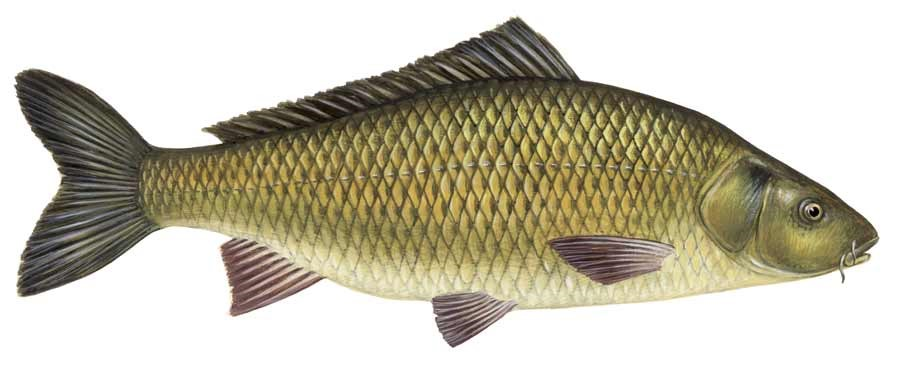
\includegraphics[width=\linewidth]{fish.jpg}
  \caption{Here is a fish.}
	\label{fig:teaser}
}

%% Uncomment below to disable the manuscript note
%\renewcommand{\manuscriptnotetxt}{}

%% Copyright space is enabled by default as required by guidelines.
%% It is disabled by the 'review' option or via the following command:
% \nocopyrightspace

\vgtcinsertpkg

%%%%%%%%%%%%%%%%%%%%%%%%%%%%%%%%%%%%%%%%%%%%%%%%%%%%%%%%%%%%%%%%
%%%%%%%%%%%%%%%%%%%%%% START OF THE PAPER %%%%%%%%%%%%%%%%%%%%%%
%%%%%%%%%%%%%%%%%%%%%%%%%%%%%%%%%%%%%%%%%%%%%%%%%%%%%%%%%%%%%%%%%

\begin{document}

%% The ``\maketitle'' command must be the first command after the
%% ``\begin{document}'' command. It prepares and prints the title block.

%% the only exception to this rule is the \firstsection command

\firstsection{Introduction}

\maketitle

Artificial intelligence has taken the world of technology by storm. Deep multilayer neural networks are being successfully applied in a wide range of applications that are regularly outperforming humans in object recognition \cite{krizhevsky_imagenet2012, simonyan_very_deep2014,szegedy2015}. 
Originally inspired by neuroscientific discoveries, the recent advances in deep learning have been the direct results of engineering efforts, more specifically in convolutional neural networks (CNNs). 
While there has been significant advancement, this does not mean we understand what CNNs are doing and we are in fact treating them as blackboxes without detracting from their success \cite{goodfellow_book, deeplearning_blackbox2017}. 
Our current knowledge of biological vision suggests that modern machine learning models indeed mimic the underlying biology by abstracting the many details of biological neural networks \cite{yamins2016using, hassabis2017neuroscience}.

Despite tremendous research efforts and generating massive datasets, we are far from fully understanding biological vision. 
Similarly, we are constantly developing inventive features for deep artificial networks without truly understanding it in its entirety. As a result, a double discrepancy is observed. 
Advances in neuroscience can revolutionize machine learning by reverse-engineering neural circuits, yielding new classifiers which, in turn, can help process the massive biological data. 
There are many existing questions which must be answered in order to fill this gap of our understanding.

We focus on perception... experiments from cleveland mcgill..



%\emph{Can we leverage decades of visualization research to understand the way convolutional neural networks process data?}
%
%Information visualization has been an established research field for decades which has resulted in numerous insightful findings in regards to how human beings can best process information visually.
%Unpublished preliminary experiments have shown that data representations customized for the human eye also can improve the performance of an automatic classifier. 
%While the reasons for this are still unknown, specified research can most certainly advance the understanding of deep neural networks.

\subsection{Biological Vision}

\begin{figure}[t]
	  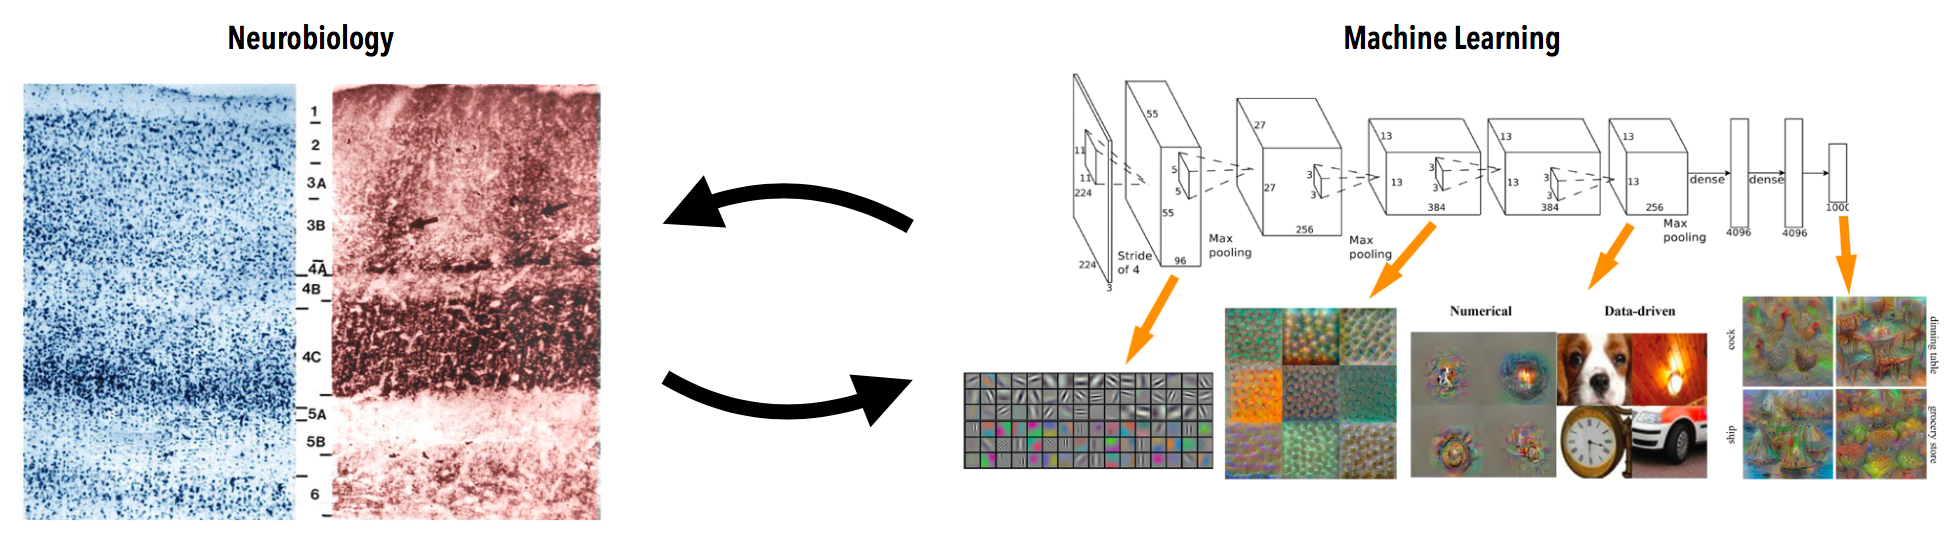
\includegraphics[width=\linewidth]{biology_vs_cnn.png}
  \caption{The Biological Vision (schematic)}
	\label{fig:vision}
\end{figure}

Biological vision is an extremely powerful system which allows humans the ability, and seemingly without effort, to recognize an enormous amount of distinct objects in the world. 
Object detection is extremely difficult and therefore is especially impressive as light intensities can change by levels of magnitude and contrast between foreground and background is so often low. 
In addition, the visual scene changes every time the human body or human eyes move. 
This visual system exhibits a very noisy structure but because it is organized by layers it has inspired the mathematical theory of multilayer neural networks. 
What is remarkable is that even though current machine learning models do not resemble the complexity of its biological pendant, they inherently generalize extremely well. 
Neural networks trained on one specific task can be used to perform detection or segmentation of, seemingly, unrelated objects with relatively minor retraining. 
The reported classification performance is superior to that of humans and the question in regards to their functionality opens an interesting research topic.


GOALS
...reduce the gap between neurobiology and data science to advance the understanding of visual cortex inspired machine learning

CONTRIBUTIONS

- experiments of cleveland mcgill with systematic parametrization and evaluation

- ranking like cleveland mcgill for machine perception?

- many other insights?

- framework





\maketitle

\section{Previous Work}

\textbf{Graphical Perception.} Cleveland and McGill~\cite{cleveland_mcgill} introduce the fundamental concept of \emph{graphical perception} and investigate how different visual attributes and encodings are perceivable by humans. They define \emph{elementary perceptual tasks} as mental-visual stimuli to understand encodings in visualizations. Based on these definitions, the authors propose and perform different experiments such as the \emph{position-angle} experiment which compares bar charts and pie charts, the \emph{position-length} experiment where users judge relations between encoded values in grouped and divided bar charts, and the \emph{bars-and-framed-rectangles} experiment to evaluate Weber's law. Heer and Bostock later reproduced the Cleveland-McGill experiments crowd-sourced on Mechanical Turk~\cite{HeerBostock2010} which lead to follow-up work from Harrison \textit{et al.}~\cite{harrison2013influencing} who replicated the experiments while observing emotional states. Both papers report similar results to Cleveland and McGill which increased our motivation to mimmick their pioneering work. Our experimental setup replicates the original setup of Cleveland and McGill - just instead of humans, we use convolutional neural networks due to the connection with the human visual system. While we focus on Cleveland and McGill's work from 1984, many other excellent articles from the last decades target low-level visual encoding~\cite{bertin1967semiologie,cleveland1985graphical,treisman1988feature, wilkinson2006grammar, carpendale2003considering,widgor_perception2007,munzner2015visualization}.

Interesting are also the rankings of correlation visualization using Weber's law~\cite{harrison2014_webers_law_rank}. This law defines the proportional relation between the initial distribution density and perceivable change. In this paper, we investigate with a simple experiment whether this holds for convolutional neural networks.
\\~\\
%\textbf{Comparing Visual Encodings.} Different visual encodings have advantages or disadvantages and the community does a great job comparing them. Higher-level comparisons include 2D versus 3D vector field and rendering studies~\cite{mckenzie_2d_3d,forsberg2009comparing_3d_vector,laidlaw_2d_vector,borkin2011arteries}, timeseries~\cite{herr2009timeseries} and scatterplots~\cite{tremmel1995visual,Wang_linegraph_vs_scatterplot}. Lower-level experiments target - besides others - open versus closed encodings~\cite{open_vs_closed_shapes}, and several evaluations of color space~\cite{ware1988color,rheingans1992color,Rogowitz2001_colormaps,kindlmann2002color}. While we investigate lower-level visual encodings in this work, we delay colorspace experiments for future work.

\textbf{Computational Visualization Understanding.}

Pineo \textit{et al.}~\cite{Pineo2012_computational_perception} create computational model of human vision based on neural networks and their experiments show that understanding visualization triggers neural activity in high-level areas of cognition. The authors suspect that this level of understanding is produced by low-level neurons performing elementary perceptional tasks. We are further investigating this suspision.
Other work tries to parse infographics by finding higher-level saliency models~\cite{bylinskii2016should}, or by extracting text or key visual elements~\cite{diagram_understanding,kembhavi2016diagram,zoya_text_visual_tags}. However, none of these works focus on computational understanding of lower-level building blocks of visualizations such as curvature, lengths, or position.
\\~\\
\textbf{Visual Cortex Inspired Machine Learning.} 
%Classifiers mimmicking the human visual system are a hot topic and many different architectures, models, and paradigms exist. Feed-forward neural networks 
The human visual cortex is an extremely powerful system which allows the ability, and seemingly without effort, to recognize an enormous amount of distinct objects in the world. This visual system is organized in layers and has inspired the theory of computational classifiers based on multilayer neural networks. Fukushima and Miyake developed the Neocognitron quantitative model~\cite{fukushima1982neocognitron} that ultimately led to the important work of Hinton, Bengio, and LeCun: \textit{deep neural networks}~\cite{lecun2015deep}, visual cortex inspired machine learning.
Nowadays, such classifiers exist with many different architectures. For this paper, we select the traditional \emph{LeNet-5}~\cite{lenet} which was designed to recognize hand-written digits, the VGG19~\cite{simonyan_very_deep2014} classifier with 16 convolutional layers, and the Xception~\cite{xception} classifier with 36 convolutional layers. Selecting these specific networks allows us to compare archtitectures with different depths.
%Object detection is extremely difficult and therefore is especially impressive as light intensities can change by levels of magnitude and contrast between foreground and background is so often low. 
%In addition, the visual scene changes every time the human body or human eyes move. 
%This visual system exhibits a very noisy structure but because it is organized by layers it has inspired the mathematical theory of multilayer neural networks. 

%In 1962 Hubel and Wiesel were the first to begin studying the visual cortex from the standpoint of a neuroscientist. Their experimental findings on cats and macaque monkeys suggested a hierarchy of cells with increasing complexity which was then later transferred to the hierarchical model of different layers. Twenty years later, this insight was translated to the Neocognitron quantitative model, by Fukushima and Miyake, which ultimately led to the important work of Hinton, Bengio, and LeCun in the 1980s. Their work on stochastic gradient descent approximation, and the availability of faster computer hardware then led to today’s deep learning networks. In the last decade, this field has exhibited rapid growth, constant evolution, and new applications in various domains.


%The reported classification performance is superior to that of humans and the question in regards to their functionality opens an interesting research topic.
%Visual cortex inspired machine learning classifiers exist with many different architectures. We select the traditional \emph{LeNet-5}~\cite{lenet} which was designed to recognize hand-written digits, the VGG19~\cite{simonyan_very_deep2014} classifier with 16 convolutional layers, and the Xception~\cite{xception} classifier with 36 convolutional layers. 
%
%What is remarkable is that even though current machine learning models do not resemble the complexity of its biological pendant, they inherently are able to generalize but only after learning thousands of examples. 
%Neural networks trained on one specific task can be used to perform detection or segmentation of, seemingly, unrelated objects with relatively minor retraining~\cite{transfer_learning}. 
%
%
%We think that the biological inspiration of modern convolutional neural networks yields the evaluation of principles of human perception with computers.
%
%
%MLP, LeNet, VGG, ImageNet, XCeption, ResNets etc and work from THomas Serre
%
%
%- https://link.springer.com/chapter/10.1007/978-3-642-14600-8_46
%
%- https://github.com/tidyverse/ggplot2/wiki/Recommended-Reading
%
%- last year's VADL workshop: https://vadl2017.github.io/




%% if specified like this the section will be committed in review mode
%\acknowledgments{
%The authors wish to thank A, B, and C. This work was supported in part by
%a grant from XYZ (\# 12345-67890).}

%\bibliographystyle{abbrv}
\bibliographystyle{abbrv-doi}
%\bibliographystyle{abbrv-doi-narrow}
%\bibliographystyle{abbrv-doi-hyperref}
%\bibliographystyle{abbrv-doi-hyperref-narrow}

\bibliography{paper.bib}
\end{document}

